\documentclass[11pt]{article}
\usepackage[a4paper,margin=2.4cm]{geometry}
\usepackage{lmodern}
\usepackage[T1]{fontenc}
\usepackage{amsmath,amssymb,amsthm}
\usepackage{booktabs}
\usepackage{graphicx}
\usepackage{xcolor}
\usepackage{enumitem}
\usepackage{caption}
\usepackage[colorlinks=true,linkcolor=blue!50!black,citecolor=blue!50!black,urlcolor=blue!50!black]{hyperref}

\newcommand{\dd}{\mathrm{d}}
\newcommand{\ee}{\mathrm{e}}
\newcommand{\Vus}{|V_{us}|}
\newcommand{\Gapp}{\Gamma_{\mathrm{app}}}
\newcommand{\Sig}{\Sigma}
\newcommand{\BR}{\mathcal{B}}
\newcommand{\Mz}{M_0}
\newcommand{\ii}{\mathrm{i}}
\newtheorem{lemma}{Lemma}
\newtheorem{prop}{Proposition}
\theoremstyle{remark}
\newtheorem*{remark}{Remark}
\captionsetup{font=small,labelfont=bf}
\setlength{\parskip}{0.4em}

\title{Certified bounds on the inclusive $\tau\to X_s\nu_\tau$ rate\\ from lattice correlators with a Hausdorff moment condition on $[-1,1]$}
\author{Draft for Wei-Lun Chen\\[0.2em]
{\small Derivations and numerics prepared with Claude (Anthropic); every step is meant to be checked by the author.}}
\date{23 October 2026}

\begin{document}
\maketitle

\begin{abstract}
The Chebyshev method for inclusive $\tau$ decays assumes that the lattice correlator is a positive
combination of $\lambda^t$ with $\lambda=\ee^{-E}\in(0,1]$. For domain-wall fermions with $M_5>1$ the
transfer matrix has negative eigenvalues, and the assumption is not guaranteed.
I show, line by line, how the rate is written as a linear functional of a positive measure,
why the old Chebyshev coefficients leave $[-1,1]$, and how a moment problem on $[-1,1]$ gives
\emph{certified} upper and lower bounds on the kernel integral from the RBC/UKQCD $48^3\times96$
and $64^3\times128$ $\bar u s$ correlators.
On these data the support $(0,1]$ is excluded at $3\sigma$ in the $J=0$ (time-component) channels,
while $[-1,1]$ is compatible. The resulting interval is $0.199\lesssim\Vus\lesssim0.250$ for a
\emph{placeholder} value of the strange branching fraction $\BR_s$; it is a guarantee under the stated assumptions,
not a precision determination.
\end{abstract}

\tableofcontents

%--------------------------------------------------------------------
\section{Introduction}
The inclusive hadronic width $\Gamma(\tau\to X_s\nu_\tau)$ gives $\Vus$ once the spectral function of the
$\bar u s$ currents is known. On the lattice only the Euclidean correlator $C(t)$ is available. The method of
Refs.~\cite{Hashimoto:2017,Bailas:2020,Gambino:2020} expands the kernel in shifted Chebyshev polynomials $T^*_n(\lambda)$ of
$\lambda=\ee^{-\hat H}$ and uses $|\langle T^*_n\rangle|\le1$, which holds for a positive measure on $[0,1]$.

Three observations motivate this note.
\begin{enumerate}[leftmargin=*,itemsep=0pt]
\item With M\"obius domain-wall fermions at $M_5=1.8$ the one-step transfer matrix has real negative eigenvalues
      \cite{Syritsyn:2007}; a positive measure on $[0,1]$ is then not guaranteed.
\item In the old direct-sum implementation the coefficients $\langle T^*_n\rangle$ leave $[-1,1]$ at $n\simeq5$--$8$
      (Sec.~\ref{sec:cheb}), and the resulting $\Vus$ does not converge with the number of terms.
\item The kernel is singular at $E\to0$ and is cut off by a regulator without physical meaning; a lower edge $E\ge M_K$ is
      physical and removes the need for it.
\end{enumerate}
The remedy proposed here keeps the structure of the calculation but replaces the support $(0,1]$ by $[-1,1]$ and replaces
the Chebyshev truncation by a moment problem whose answer is an \emph{interval}.

\paragraph{Conventions.} $E$ is an energy, $\lambda=\ee^{-E}$. Lattice quantities carry no unit (a hat when ambiguity is possible);
$a^{-1}$ converts to GeV. $T$ is the number of correlator values used, $t=1,\dots,T$.
%--------------------------------------------------------------------
\section{From the decay rate to a linear functional of the correlator}
\subsection{The rate}
Following your note (Eq.~(28)), with $y=Q^2/m_\tau^2$ and $\Gamma_0=m_\tau^5G_F^2/(192\pi^3)$,
\begin{equation}
 R\equiv\frac{\Gamma}{\Gamma_0}=12\pi^2|V_{us}|^2S_{EW}\int_0^{m_\tau^2}\frac{\dd Q^2}{m_\tau^2}(1-y)^2\Big[(1+2y)\rho^{(1)}(Q^2)+\rho^{(0)}(Q^2)\Big].
\end{equation}
Multiplying by $\Gamma_0$ and using $12\pi^2/(192\pi^3)=1/(16\pi)$,
\begin{align}
 \Gamma(\tau\to X_s\nu)&=\Vus^2\,S_{EW}\,\frac{G_F^2m_\tau^3}{16\pi}\;\Gapp,\\
 \Gapp&\equiv\int_0^{m_\tau^2}\dd Q^2\Big[K_1(y)\rho^{(1)}(Q^2)+K_0(y)\rho^{(0)}(Q^2)\Big],\\
 K_1(y)&=(1-y)^2(1+2y)\,\theta(1-y),\qquad K_0(y)=(1-y)^2\,\theta(1-y).
\end{align}
This is Eq.~(44) of your note with $\Gamma_{\rm Exp}\to\BR_s\Gamma_\tau$ in the numerator.

\paragraph{Check with the kaon pole.} Take $\rho^{(0)}=f_K^2\delta(Q^2-M_K^2)$ (your Eq.~(25)). Then
$\Gapp=f_K^2K_0(M_K^2/m_\tau^2)=f_K^2(1-M_K^2/m_\tau^2)^2$, which reproduces Eq.~(26),
$\Gamma(\tau\to K\nu)=G_F^2f_K^2m_\tau^3(1-M_K^2/m_\tau^2)^2|V_{us}|^2/(16\pi)$.
The $K^*$ with $\rho^{(1)}=f_{K^*}^2\delta(Q^2-M_{K^*}^2)$ gives $f_{K^*}^2(1-y)^2(1+2y)$, Eq.~(27).

\subsection{Spectral representation of the correlator}
Your Eq.~(29) is
\begin{equation}
 C(t)=\int_0^\infty\dd Q\,Q^2\rho(Q^2)\,\ee^{-Qt}\;\equiv\;\int_0^\infty\dd E\,\rho_E(E)\,\ee^{-Et},\qquad \rho_E(E)=E^2\rho(E^2).
 \label{eq:spec}
\end{equation}
The overall normalisation is fixed by the one-state case, Eqs.~(48) and (51) of your note: a single state of mass $M$ and
decay constant $f$ gives the renormalised, per-volume correlator
\begin{equation}
 C_{\rm ren}(t)\equiv\frac{Z^2\,C_{\rm file}(t)}{L^3}=\frac{Mf^2}{2}\,\ee^{-Mt},
 \qquad f=Z\sqrt{\frac{2A}{ML^3}}\ \ (C_{\rm file}\simeq A\ee^{-Mt}),
 \label{eq:norm}
\end{equation}
i.e.\ $\rho_E=\tfrac12Mf^2\delta(E-M)$. With $\delta(E-M)=2M\,\delta(E^2-M^2)$ this is
$\rho(Q^2)=\rho_E/E^2=f^2\delta(Q^2-M^2)$, consistent with Eq.~(25). The general case follows by linearity. Here $Z=Z_A=Z_V$ (your Tables~2--4).

\subsection{Rewriting $\Gapp$ in the energy variable}
Substitute $Q^2=E^2$, $\dd Q^2=2E\,\dd E$ in $\Gapp$ and use $\rho(E^2)=\rho_E(E)/E^2$:
\begin{equation}
 \int\dd Q^2K(Q^2)\rho(Q^2)=\int\dd E\,2E\,K\,\frac{\rho_E(E)}{E^2}=\int_0^\infty\dd E\;\frac{2}{E}\,K(E)\,\rho_E(E).
 \label{eq:Gapp_E}
\end{equation}
\emph{Check:} $\rho_E=\tfrac12Mf^2\delta(E-M)$ gives $\frac{2}{M}\frac12Mf^2K=f^2K$, as it must.

\subsection{Lattice units}
Let $\hat E=aE$ and let $c(t)=Z^2C_{\rm file}/L^3$ be the correlator in lattice units, $c(t)=\int\dd\hat E\,\hat\rho(\hat E)\ee^{-\hat Et}$.
For one state $\hat M=aM$ and $\hat f=af$ in Eq.~(\ref{eq:norm}). Then, with $\hat\Sigma\equiv\int\dd\hat E\,(2/\hat E)K\,\hat\rho$,
\begin{equation}
 \hat\Sigma=\hat f^2K=a^2f^2K=a^2\,\Gapp
 \qquad\Longrightarrow\qquad \Gapp=(a^{-1})^2\,\hat\Sigma .
 \label{eq:units}
\end{equation}
By linearity this holds for any $\hat\rho$. \emph{It is $(a^{-1})^2$, not $(a^{-1})^3$}; $K$ is evaluated at
$y=(a^{-1}\hat E)^2/m_\tau^2$, so the kernel edge sits at $\hat E=m_\tau a=1.027$ (48I) and $0.753$ (64I).

\subsection{Which component carries $J=0$ and which $J=1$}
Write the vacuum polarisation as
$\Pi^{\mu\nu}(q)=(q^\mu q^\nu-q^2g^{\mu\nu})\Pi^{(1)}+q^\mu q^\nu\Pi^{(0)}$. At zero spatial momentum $q=(q^0,\vec0)$:
\begin{align}
 \Pi^{00}&=(q_0^2-q^2)\Pi^{(1)}+q_0^2\Pi^{(0)}=q_0^2\,\Pi^{(0)}\qquad(q^2=q_0^2),\\
 \Pi^{ii}&=-q^2g^{ii}\,\Pi^{(1)}=q^2\,\Pi^{(1)}\qquad(\text{no sum over } i,\ g^{ii}=-1).
\end{align}
Hence the temporal components ($A_T=\gamma_5\gamma_4$, $V_T=\gamma_4$) carry $J=0$ and the spatial ones, averaged over $i$,
($A_S$, $V_S$) carry $J=1$:
\begin{equation}
 \Sig_{\rm tot}=\sum_{X\in\{A,V\}}\Big[\Sig^{(0)}_{X_T}+\Sig^{(1)}_{X_S}\Big],\qquad
 \Sig^{(J)}_{c}=(a^{-1})^2\!\int\!\dd\hat E\,\frac{2}{\hat E}K_J\,\hat\rho_c .
 \label{eq:channels}
\end{equation}
In the RBC files the eight gamma matrices are $g=1,2,4\to V_{x,y,z}$, $8\to V_T$, $14,13,11\to A_{x,y,z}$, $7\to A_T$.
\emph{Remark.} The old \texttt{vus()} assigns $J=1$ to both axial terms and $J=0$ to both vector terms, which disagrees with Eq.~(\ref{eq:channels}) and with
the mock code in the same file.

%--------------------------------------------------------------------
\section{The support of the spectral measure}
\subsection{Positive transfer matrix}
If the one-step transfer matrix $\hat T=\ee^{-\hat H}$ is Hermitian and positive, with eigenvalues $\lambda_n=\ee^{-E_n}\in(0,1]$ and overlaps
$c_n=\langle n|J|0\rangle$,
\begin{equation}
 C(t)=\sum_n|c_n|^2\lambda_n^{\,t}=\int\dd\nu(\lambda)\,\lambda^t,\qquad \nu\ge0,\ \ \mathrm{supp}\,\nu\subset(0,1].
\end{equation}
This is the hypothesis behind the shifted-Chebyshev method.

\subsection{$M_5>1$}
Syritsyn and Negele \cite{Syritsyn:2007} construct $\hat T$ for Shamir domain-wall fermions: its eigenvalues are real,
and negative ones appear for $M_5>1$. They do not discuss the sign of the weights. If only link reflection positivity holds,
the natural form is
\begin{equation}
 C(t)=\sum_n|c_n|^2\lambda_n^{\,t-1}=\int\dd\sigma(\lambda)\,\lambda^{t-1},\qquad t\ge1,\qquad \sigma=\sum_n|c_n|^2\delta_{\lambda_n}\ge0,
 \quad \mathrm{supp}\,\sigma\subset[-1,1].
 \label{eq:model}
\end{equation}
Define the moments $m_k\equiv\int\dd\sigma\,\lambda^k=C(k+1)$, $k=0,1,\dots$ ($C(0)$ is dropped: contact terms).
For $\lambda>0$ the relation to the spectral density is $\dd\sigma=\lambda\hat\rho\,\dd\hat E$, because
$\int\hat\rho\,\ee^{-\hat Et}\dd\hat E=\int\lambda^{t-1}(\lambda\hat\rho\,\dd\hat E)$. States with $\lambda<0$ carry
$\sigma\ge0$ in this convention (a negative weight in $C(t)=\int\lambda^t\,\dd\nu$ with $\dd\nu=\dd\sigma/\lambda$).

\paragraph{Hypotheses.} $H_{[0,1]}$: $\mathrm{supp}\,\sigma\subset(0,1]$ (old). $H_{[-1,1]}$: $\mathrm{supp}\,\sigma\subset[-1,1]$ (new).
$H_{[-1,1]}$ is weaker, contains $H_{[0,1]}$, and is \emph{not proven} for $M_5=1.8$ M\"obius fermions; it can only be tested.

\paragraph{Parity of the start time.} For the sequence $s_k=C(t_s+k)=\int\dd\sigma\,\lambda^{t_s-1}\lambda^k$ to be moments of a positive measure
on $[-1,1]$ we need $\lambda^{t_s-1}\ge0$ there, i.e.\ $t_s-1$ even, $t_s$ odd. For even $t_s$ the negative-$\lambda$ states enter with negative weight.
The old method normalises with $2t_0=1$, an odd $t_s$.

%--------------------------------------------------------------------
\section{Testing the hypothesis: Hausdorff positivity}
\subsection{Necessary conditions, proved}
Let $P(\lambda)=\sum_{i=0}^nx_i\lambda^i$ be a real polynomial and $s_k=\int\dd\sigma\,\lambda^k\,\lambda^{t_s-1}$. If $\sigma\ge0$ on $[-1,1]$:
\begin{align}
 x^{\!\top}H x&=\sum_{ij}x_ix_j\,s_{i+j}=\int\dd\sigma\,\lambda^{t_s-1}P(\lambda)^2\ \ge0,
 &H_{ij}&=s_{i+j},\label{eq:H0}\\
 x^{\!\top}H^{\rm loc}x&=\int\dd\sigma\,\lambda^{t_s-1}(1-\lambda^2)P(\lambda)^2\ \ge0,
 &H^{\rm loc}_{ij}&=s_{i+j}-s_{i+j+2}.\label{eq:Hloc}
\end{align}
For support $[0,1]$ the second matrix is $H^{\rm loc}_{ij}=s_{i+j+1}-s_{i+j+2}$, from the weight $\lambda(1-\lambda)$.
Schm\"udgen \cite{Schmudgen:2020} proves that for $s_0,\dots,s_{2n}$ these conditions are also \emph{sufficient}
(no rank condition on a compact interval). We only need necessity: a significantly negative eigenvalue \emph{excludes} the hypothesis;
passing means compatibility, not proof.

\subsection{Scaling and statistics}
Scaling $H\to D^{-1}HD^{-1}$ with $D=\mathrm{diag}(\sqrt{|H_{ii}|})$ is a congruence and does not change positive semidefiniteness (Sylvester's law),
and removes the strong decay of $s_k$. For each $(t_s,n)$ we compute the smallest eigenvalue $\mu_{\min}$ and its jackknife error over configurations, and
call a matrix a \emph{violation} if $\mu_{\min}/\sigma<-3$, a \emph{pass} if $>3$.
(The rows of the data files carry no configuration label; the autocorrelation along the row order is at the noise level,
$|{\rm ac}|<0.05$ for lags $1$--$100$, so the jackknife error does not depend on the assumed ordering.)

\subsection{Result}
\begin{table}[h]
\centering\small
\begin{tabular}{llcc}
\toprule
channel & support & odd $t_s$ (pass/inc/viol) & even $t_s$ \\
\midrule
$V_S$, $A_S$ ($J=1$), 48I and 64I & $[-1,1]$ & 5--7 / 1--3 / 0 & 4--6 / 2--4 / 0 \\
$V_T$ ($J=0$), 64I & $[-1,1]$ & 5/3/0 & 2/3/\textbf{3} \\
$V_T$ ($J=0$), 64I & $[0,1]$ & 0/5/\textbf{3} & 3/5/0 \\
$A_T$ ($J=0$), 64I & $[-1,1]$ & 5/3/0 & 3/3/2 \\
$A_T$ ($J=0$), 64I & $[0,1]$ & 3/3/\textbf{2} & 3/5/0 \\
\bottomrule
\end{tabular}
\caption{Localizing matrices, $n\ge2$, $t_s\le8$. At odd $t_s$ the support $[-1,1]$ is never violated in any channel on either ensemble;
the $J=0$ channels show the pattern expected for negative-$\lambda$ states. Full table: \texttt{hankel\_scan.py}.}
\label{tab:hankel}
\end{table}
The $J=0$ channels violate $[0,1]$ at odd $t_s$ and $[-1,1]$ at even $t_s$, as predicted by Eq.~(\ref{eq:model}).
The $J=1$ channels do not discriminate. Because the same data enter many $(t_s,n)$ tests, isolated $3\sigma$ violations are expected by chance;
$V_T$ is also the least clean channel (a non-conserved local current for $m_u\ne m_s$).

%--------------------------------------------------------------------
\section{The Chebyshev coefficients}\label{sec:cheb}
\subsection{Definitions and the old relation}
With $\lambda=(1+\cos\theta)/2=\cos^2(\theta/2)$ set $T^*_j(\lambda)=\cos j\theta=T_j(2\lambda-1)$.
Normalise $\bar C(t)=C(t+2t_0)/C(2t_0)=m_t/m_0\equiv\langle\lambda^t\rangle$. Then
\begin{align}
 \lambda^t&=\cos^{2t}\!\tfrac\theta2=2^{-2t}\!\!\sum_{k=0}^{2t}\binom{2t}{k}\ee^{\ii(t-k)\theta}
 =2^{1-2t}\Big[\tfrac12\binom{2t}{t}+\sum_{j=1}^{t}\binom{2t}{t-j}\cos j\theta\Big],\\
 \bar C(t)&=2^{1-2t}\Big[\tfrac12\binom{2t}{t}+\sum_{j=1}^{t}\binom{2t}{t-j}\langle T^*_j\rangle\Big],\label{eq:cbar}
\end{align}
which is your Eq.~(56) (with $\langle T^*_0\rangle=1$ by normalisation). The old method fits $\langle T^*_j\rangle$ to $\bar C(t)$, $t=1,\dots,T$, with the
prior $|\langle T^*_j\rangle|<1$ (through $\mathrm{erfinv}$).
\subsection{The bound, and when it fails}
\begin{lemma}
If $\sigma\ge0$ is normalised on $[0,1]$, $|\langle T^*_n\rangle|\le1$. If $\sigma\ge0$ is normalised on $[-1,1]$, $|\langle T_n\rangle|\le1$.
\end{lemma}
\begin{proof}
$|T^*_n|\le1$ on $[0,1]$ and $|T_n|\le1$ on $[-1,1]$, so $|\langle T\rangle|\le\int|T|\,\dd\sigma\le\int\dd\sigma=1$.
\end{proof}
Now let a weight $w$ sit at $\lambda=-\varepsilon$ ($\varepsilon>0$). Since $2\lambda-1=-1-2\varepsilon<-1$,
\begin{equation}
 T^*_n(-\varepsilon)=(-1)^n\cosh\!\big(n\,\mathrm{arccosh}(1+2\varepsilon)\big)\simeq\tfrac12(-1)^n\ee^{\,n\kappa},\quad \kappa=\mathrm{arccosh}(1+2\varepsilon),
\end{equation}
so the contribution $w\,T^*_n(-\varepsilon)$ exceeds $1$ for $n\gtrsim\ln(2/w)/\kappa$. For $\varepsilon=0.1$ ($\kappa=0.62$):
$n\gtrsim8.5$ for $w=1\%$ and $n\gtrsim4.8$ for $w=10\%$. A small negative-$\lambda$ component is therefore enough to push the old
coefficients out of $[-1,1]$ at the $n$ observed in the data.

\subsection{Noise amplification}
The coefficients of $T^*_n(x)$ alternate in sign (all roots lie in $(0,1)$, Descartes), so $\sum_k|c_k|=|T^*_n(-1)|=T_n(3)\simeq\tfrac12(3+2\sqrt2)^n$.
The coefficients of $T_n(x)$ alternate in $x^2$, so $\sum_k|c_k|=|T_n(\ii)|\simeq\tfrac12(1+\sqrt2)^n$. At $n=12$ these are $7.7\times10^{8}$ and
$2.0\times10^{4}$: the $[-1,1]$ basis amplifies the statistical noise of the moments $\sim4\times10^4$ times less.
The price is a coarser resolution in $\lambda$ (about a factor $2$ in the polynomial degree).

\subsection{Data}
\begin{figure}[h]
\centering
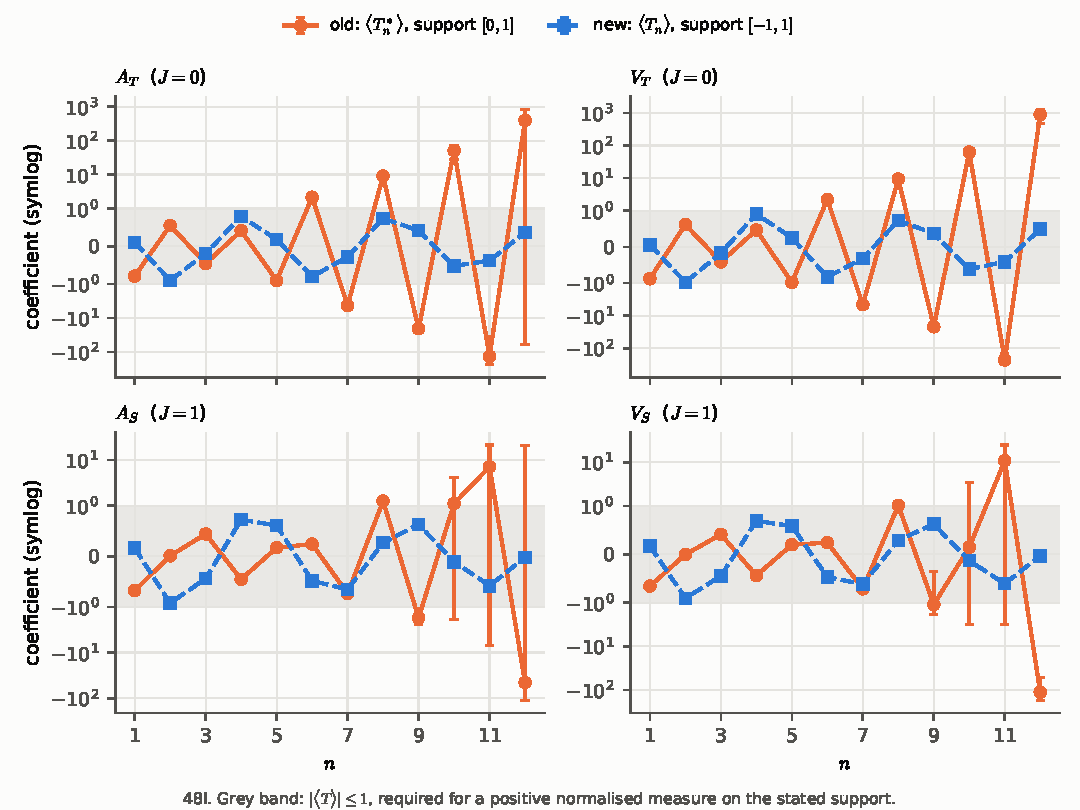
\includegraphics[width=0.92\textwidth]{figs/fig_cheb.pdf}
\caption{$\langle T^*_n\rangle$ (old, orange) and $\langle T_n\rangle$ (new, blue) on 48I, four channels, jackknife errors; symmetric-log axis; the grey band is $[-1,1]$.
The old coefficients leave the band at $n=5$--$8$ (e.g.\ $A_T$, $n=6$: $2.16\pm0.04$) and reach $10^2$--$10^3$ at $n=12$.
The new ones stay inside for all channels and $n\le12$ (maximum $0.98$, error $\le0.02$). They follow $\cos(n\pi/2)$ because the measure sits near $\lambda=0$, so this is a necessary, weak test.}
\end{figure}

%--------------------------------------------------------------------
\section{Certified bounds}
\subsection{The problem}
Per channel $c$ with kernel $J$, let $\kappa_J(\lambda)=\frac{2}{E}K_J\big((a^{-1}E)^2/m_\tau^2\big)$ with $E=-\ln\lambda$. From
Eqs.~(\ref{eq:channels}) and $\dd\sigma=\lambda\hat\rho\,\dd\hat E$,
\begin{equation}
 \hat\Sigma_c=\int\dd\sigma(\lambda)\,g(\lambda),\qquad g(\lambda)=\begin{cases}\kappa_J(\lambda)/\lambda,&0<\lambda\le\ee^{-M_0}\\ 0,&\lambda<0.\end{cases}
 \label{eq:g}
\end{equation}
States with $\lambda<0$ are lattice artefacts: they contribute nothing to the physical rate but they consume the moment budget. The lower edge $E\ge M_0$
(the kaon, the lightest $\bar us$ state) is necessary because $g\sim2/E$ diverges at $E\to0$.
Bounds are sought for all positive measures consistent with the data:
\begin{equation}
 \hat\Sigma^{\pm}=\ \sup/\inf\ \int g\,\dd\sigma\quad\text{s.t.}\quad \sigma\ge0\ \text{on}\ S,\quad |m_k-C(k+1)|\le z\,\delta_{k+1},\ \ k=0,\dots,T-1,
 \label{eq:primal}
\end{equation}
with $S=[-1,\ee^{-M_0}]$ (new) or $(0,\ee^{-M_0}]$ (old), and $\delta_t$ the jackknife error of $C(t)$.

\subsection{Weak duality (the certificate)}
\begin{prop}
Let $p(\lambda)=\sum_{k=0}^{T-1}p_k\lambda^k$ satisfy $p\ge g$ on $S$. Then for every $\sigma$ feasible in (\ref{eq:primal})
\begin{equation}
 \int g\,\dd\sigma\ \le\ \sum_kp_kC(k+1)+z\sum_k|p_k|\,\delta_{k+1}.
\end{equation}
\end{prop}
\begin{proof}
$\int g\,\dd\sigma\le\int p\,\dd\sigma=\sum_kp_km_k$ (since $\sigma\ge0$ and $p\ge g$). Write $m_k=C(k+1)+\epsilon_k$ with $|\epsilon_k|\le z\delta_{k+1}$;
then $\sum p_k\epsilon_k\le z\sum|p_k|\delta_{k+1}$.
\end{proof}
The lower bound is the mirror image with a polynomial $q\le g$ and $-z\sum|q_k|\delta_{k+1}$.
Minimising the right-hand side over $p$ is the dual of (\ref{eq:primal}); strong duality holds for the moment problem on a compact set, and for polynomial $g$ the condition $p-g\ge0$ on $[-1,1]$ is equivalent to
$p-g=s_0+(1-\lambda^2)s_1$ with sums of squares $s_0,s_1$ (Luk\'acs), i.e.\ a semidefinite program.

\subsection{Numerics and what is rigorous}
$g$ is not a polynomial, so I solve the primal on a fine grid of $\lambda$ (about $6\times10^3$ points, variables $u_i\ge0$ rescaled by $C(1)$, \texttt{scipy.optimize.linprog}/HiGHS).
This gives an \emph{inner} approximation. The dual variables $y^\pm_k$ of the two inequality rows of moment $k$ give $p_k=(y^+_k-y^-_k)/\delta_{k+1}$ with $p\ge g$ on the grid.
\emph{The rigorous step:} $p-g$ is evaluated on a dense grid of $2\times10^5$ points of the whole support, $p$ is lifted by the largest violation $\Delta$ ($p_0\to p_0+\Delta$),
and the proposition is applied. On the data the certified and the grid bounds differ by at most $3\times10^{-5}\,\mathrm{GeV}^2$ (Table~\ref{tab:bounds}).
(The check on a dense grid is numerical, not an analytic proof of $p\ge g$; $g$ is smooth and the lift is small.)

\paragraph{Statistical meaning.} Each box is $\pm z\delta_t$. With Gaussian errors the $T$ boxes jointly contain the truth with probability at least
$1-T\cdot0.0027$ for $z=3$ (Bonferroni): $\ge95\%$ for $T=18$. The covariance between $t$ is not used.

\paragraph{Calibration.} A single state ($m=0.4937$\,GeV, $f=0.1564$\,GeV on 48I, errors $10^{-3}$) gives $\Sigma\in[0.02075,0.02089]\,\mathrm{GeV}^2$
for both supports, around the exact $f^2(1-M^2/m_\tau^2)^2=0.02083$; the certificate reproduces the grid bound to $5$ digits.

\subsection{Feasibility}
The LP minimising $\max_t|\sum_i w_i\lambda_i^{t-1}-C(t)|/\delta_t$ gives the smallest $z^*$ at which a positive measure on $S$ reproduces the data.
\begin{table}[h]
\centering\small
\begin{tabular}{lcccc}
\toprule
$z^*$ at $T=14$ (old $[0,1]$ / new $[-1,1]$) & $A_T$ & $V_T$ & $A_S$ & $V_S$\\
\midrule
48I & 3.28 / 0.09 & 5.22 / 0.07 & 0.64 / 0.39 & 0.27 / 0.20\\
64I & 9.06 / 0.06 & 18.72 / 0.08 & 0.75 / 0.10 & 0.78 / 0.05\\
\bottomrule
\end{tabular}
\caption{Minimal tolerance (in $\sigma$) for the data to be reproduced by a positive measure. For $T\ge6$ the $J=0$ channels need $z^*>3$ with the old support.}
\end{table}
At $z=3$ the old support is therefore \emph{infeasible} for $A_T$ and $V_T$, at both lattice spacings and for every $T\ge6$,
which is the moment-problem version of ``the Chebyshev coefficients exceed 1''.

%--------------------------------------------------------------------
\section{Results}
\subsection{Channel bounds}
\begin{table}[h]
\centering\small
\begin{tabular}{lcccc}
\toprule
$\hat\Sigma$ bounds [GeV$^2$], $T=18$, $z=3$, certified & $A_T$ & $V_T$ & $A_S$ & $V_S$\\
\midrule
48I new $[-1,1]$ & [0.02048, 0.02119] & [0.00039, 0.00135] & [0.01021, 0.02894] & [0.03764, 0.05907]\\
64I new $[-1,1]$ & [0.02048, 0.02125] & [0.00038, 0.00127] & [0.00617, 0.02761] & [0.03653, 0.05876]\\
old $[0,1]$      & \multicolumn{2}{c}{infeasible} & \multicolumn{2}{c}{feasible, slightly tighter lower bounds}\\
\bottomrule
\end{tabular}
\caption{Certified bounds per channel. The kaon pole alone gives $f_K^2(1-M_K^2/m_\tau^2)^2=0.02084$, inside the $A_T$ interval:
the normalisation of Sec.~2 is confirmed on real data.
Certified and grid bounds differ by at most $3\times10^{-5}$\,GeV$^2$.}
\label{tab:bounds}
\end{table}
\begin{figure}[h]
\centering
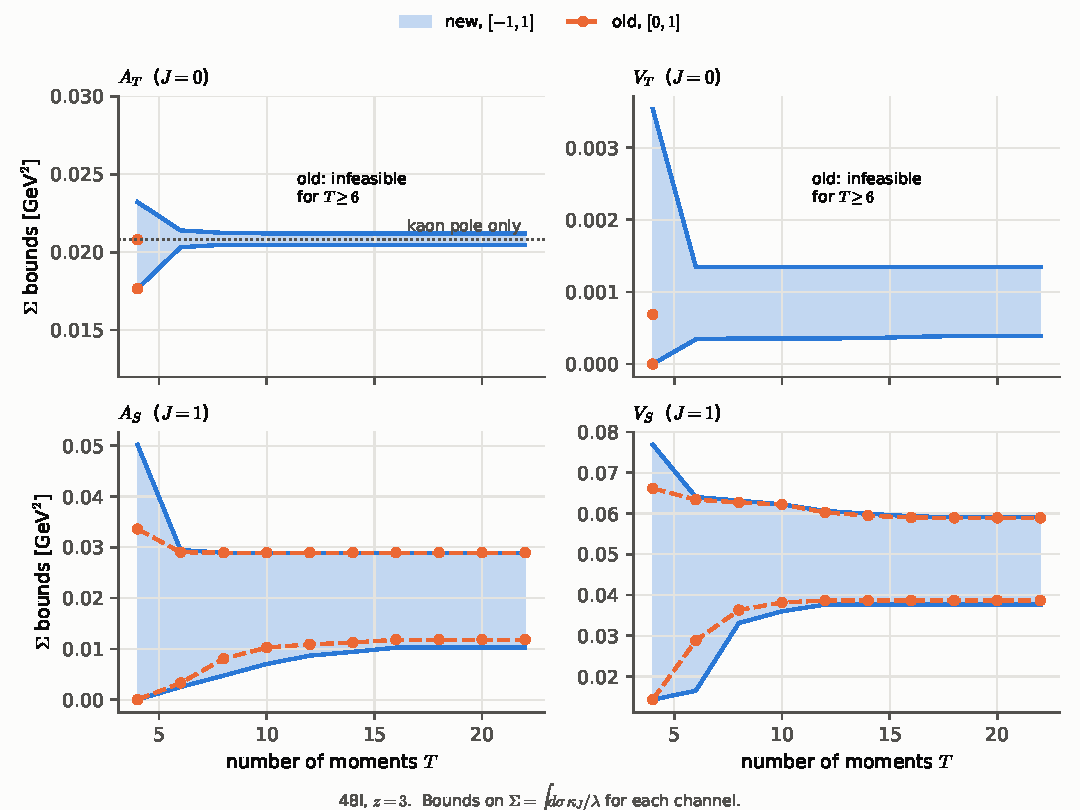
\includegraphics[width=0.92\textwidth]{figs/fig_bounds.pdf}
\caption{Bounds on $\hat\Sigma$ versus the number of moments $T$ (48I, $z=3$). New support: blue band. Old support: orange dashed, where feasible; infeasible for $A_T$, $V_T$ from $T=6$.
Beyond $T\approx18$ the relative error of $C(t)$ exceeds $25\%$ and the bounds no longer improve. The $J=1$ axial channel is the loosest.}
\end{figure}

\subsection{$\Vus$}
Eq.~(44) with $\Gamma_{\rm Exp}=\BR_s\Gamma_\tau$ gives
\begin{equation}
 \Vus=\sqrt{\frac{\BR_s\,\Gamma_\tau}{S_{EW}\,\dfrac{G_F^2m_\tau^3}{16\pi}\ \Sigma_{\rm tot}}},\qquad
 \Sigma_{\rm tot}=\sum_{c}\Sigma_c^{\pm},
\end{equation}
with $\Gamma_\tau=\hbar/\tau_\tau=2.267\times10^{-12}$\,GeV, $S_{EW}=1.0201$, $G_F^2m_\tau^3/(16\pi)=1.518\times10^{-11}\,\mathrm{GeV}^{-1}$. Bounds of the four independent channels add,
which is conservative. Then $\Vus\in[\sqrt{c/\Sigma^+_{\rm tot}},\sqrt{c/\Sigma^-_{\rm tot}}]$ with $c=\BR_s\Gamma_\tau/(S_{EW}G_F^2m_\tau^3/16\pi)$.
\begin{table}[h]
\centering\small
\begin{tabular}{llccc}
\toprule
ensemble & support & $\Sigma_{\rm tot}$ [GeV$^2$] & $\Vus$ & width\\
\midrule
48I & old $[0,1]$ & infeasible & --- & ---\\
64I & old $[0,1]$ & infeasible & --- & ---\\
48I & new $[-1,1]$ & [0.0687, 0.1105] & [0.1970, 0.2498] & 11.8\%\\
64I & new $[-1,1]$ & [0.0636, 0.1089] & [0.1985, 0.2597] & 13.4\%\\
\multicolumn{2}{l}{both ensembles, overlap ($z=3$)} & & \textbf{[0.1985, 0.2498]} & \\
\multicolumn{2}{l}{both ensembles, overlap ($z=2$)} & & [0.2006, 0.2360] & \\
\bottomrule
\end{tabular}
\caption{$T=18$. \textbf{$\BR_s=0.0293$ is a placeholder from memory, not verified; $\Vus\propto\sqrt{\BR_s}$.} The $48$I and $64$I intervals are not combined into one fit.
The value $\Sigma_{\rm tot}=0.0852$\,GeV$^2$ that corresponds to $\Vus=0.2243$ with this $\BR_s$ lies inside both intervals.}
\end{table}

\subsection{Comparison with the old direct fit}
Figure~\ref{fig:vus} shows the certified interval versus $T$ together with the values from the original code (run unchanged except for removing \texttt{cupy}), for both
kernel assignments of Sec.~2.5. The old values change by $\pm30\%$ between consecutive $T$ and their quoted errors ($\approx6\times10^{-4}$) do not include the truncation error.
\begin{figure}[h]
\centering
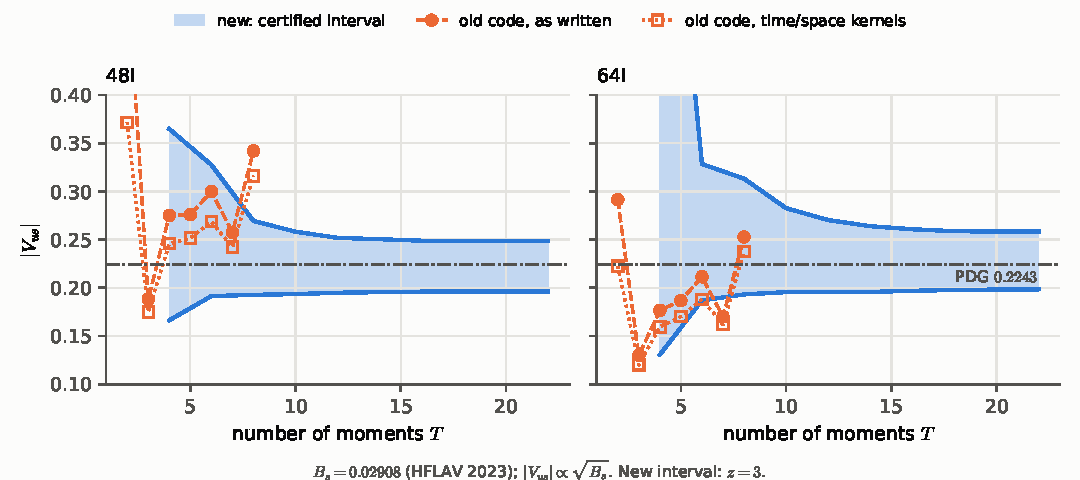
\includegraphics[width=0.96\textwidth]{figs/fig_vus.pdf}
\caption{$\Vus$ from the original code (orange; filled: as written, open: time/space kernels) and the certified interval (blue), versus $T$.
$\BR_s$ is a placeholder.}
\label{fig:vus}
\end{figure}
Points to check in the old code (details in \texttt{OLD\_CODE\_NOTES.md}): the kernel assignment, the ignored \texttt{--t0} (the argument lands in \texttt{ND}), the absence of $\BR_s$ in the
$\Vus$ formula, and the position of $Z_A^2$ (it should multiply $\Sigma$; in the code it divides inside the square root).

%--------------------------------------------------------------------
\section{What is and is not shown}
\begin{itemize}[leftmargin=*,itemsep=1pt]
\item The $(0,1]$ support is \emph{excluded} by the $J=0$ data at $\ge3.3\sigma$ (48I) and $\ge9\sigma$ (64I); $[-1,1]$ is compatible. This does not depend on any $\Vus$ number.
\item The interval is wide ($\approx\pm11\%$). It is a guarantee, not a competitive determination; the $J=1$ axial channel limits it.
\item It is valid only if (i) $\sigma\ge0$ on $[-1,1]$ holds for this action (tested at odd $t_s$, not proven), (ii) the lowest state is the kaon, (iii) $\BR_s$, $Z$, $a^{-1}$, $M_0$ are correct,
      (iv) the Gaussian error model holds. With $z=3$ and $T=18$ the statistical confidence is $\ge95\%$.
\item Not included: continuum extrapolation (one lattice spacing each), the errors of $a^{-1}$ ($\approx0.2\%$ on $\Vus$) and $Z$, the full covariance (boxes are used), lattice artefacts of the local currents,
      finite-volume effects beyond the positivity of the measure.
\item Next steps: an exact free-field M\"obius check at $M_5=1.8$ (a single negative pivot would be decisive); the experimental $\BR_s$; a SOS/SDP implementation with the exact (non-grid) polynomial certificate;
      the full covariance as an ellipsoid constraint.
\end{itemize}

%--------------------------------------------------------------------
\appendix
\section{Reproducing the numbers}
All code is in \texttt{hausdorff/} of the repository; run from the directory that contains \texttt{RBCQCD/}.
\begin{center}\small
\begin{tabular}{ll}
\toprule
\texttt{hankel\_scan.py} & Hausdorff positivity scan (Table~\ref{tab:hankel})\\
\texttt{cheb\_report.py} & $\langle T^*_n\rangle$ and $\langle T_n\rangle$ (Fig.~1)\\
\texttt{bounds\_report.py}, \texttt{bounds\_T.py} & feasibility $z^*$ and bounds versus $T$\\
\texttt{vus\_interval.py}, \texttt{vus\_certified.py} & channel sums, certificate check, $\Vus$ interval (\texttt{BS=...} sets $\BR_s$)\\
\texttt{safe\_vus.py} & library and single-state calibration (\texttt{python safe\_vus.py})\\
\texttt{old\_code\_check/} & the original \texttt{AllClass.py} run without \texttt{cupy}\\
\texttt{paper/make\_figs.py} & figures\\
\bottomrule
\end{tabular}
\end{center}
Parameters: 48I: $a^{-1}=1.7295$\,GeV, $Z=0.71076$, $M_0=0.28816$, $L=48$, $N_t=96$, 88 configurations $\times$ 48 sources;
64I: $a^{-1}=2.3586$\,GeV, $Z=0.74293$, $M_0=0.21539$, $L=64$, $N_t=128$, 40 $\times$ 64 (the split is inferred from the row count; the Hankel scan gives identical verdicts for $40\times64$ and $80\times32$).

\begin{thebibliography}{9}
\bibitem{Syritsyn:2007} S.~Syritsyn, J.~W.~Negele, \emph{Oscillatory terms in the domain wall transfer matrix}, PoS LATTICE2007 (2007) 078, arXiv:0710.0425.
\bibitem{Schmudgen:2020} K.~Schm\"udgen, \emph{Ten lectures on the moment problem}, arXiv:2008.12698.
\bibitem{Hashimoto:2017} S.~Hashimoto, PTEP 2017 (2017) 053B03, arXiv:1703.01881.
\bibitem{Bailas:2020} G.~Bailas, S.~Hashimoto, T.~Ishikawa, PTEP 2020 (2020) 043B07, arXiv:2001.11779.
\bibitem{Gambino:2020} P.~Gambino, S.~Hashimoto, Phys.\ Rev.\ Lett.\ 125 (2020) 032001, arXiv:2005.13730.
\bibitem{Boyle:2018} P.~Boyle et al., Phys.\ Rev.\ Lett.\ 121 (2018) 202003, arXiv:1803.07228.
\bibitem{RBC:2016} T.~Blum et al.\ (RBC/UKQCD), Phys.\ Rev.\ D 93 (2016) 074505, arXiv:1411.7017.
\bibitem{Abbott:2025} Abbott, Jay, Oare, arXiv:2508.01377.
\end{thebibliography}
\end{document}
